\section{Test mit Distanzklauseln} % 80 - 83
\label{sec:test_distanz}

In diesem Test werden zusätzlich zu den Basisklauseln die Klauseln aus Tabelle  \ref{fig:additional_clauses_clean} mit einbezogen.
Die Ergebnisse sind in Abbildung \ref{fig:data_dist} dargestellt.
Auch hier reduziert sich die Testlaufzeit. Im Vergleich zu den modulspezifischen Klauseln reduziert sich die Laufzeit nur um 20\%
anstatt 50\%. Genau entgegen gesetzt ist jedoch das Verhalten bezüglich der Anzahl der unterschiedlichen Lösungen. Diese Klauseln
führen dazu, dass mehr geraten und weniger berechnet wird. Wie auch bei den Basisklauseln lässt sich in der Variante ohne XOR-Klauseln
ein Sprung der Lautzeit nach oben erkennen. Dieser erfolgt bei diesem Test jedoch erst bei 17 Bit.
\begin{figure}[!h]
  \centering
  \begin{minipage}[c]{0.45\textwidth}
  \begin{flushleft}Gesamtdauer ohne XOR: 155:31:37\end{flushleft}
  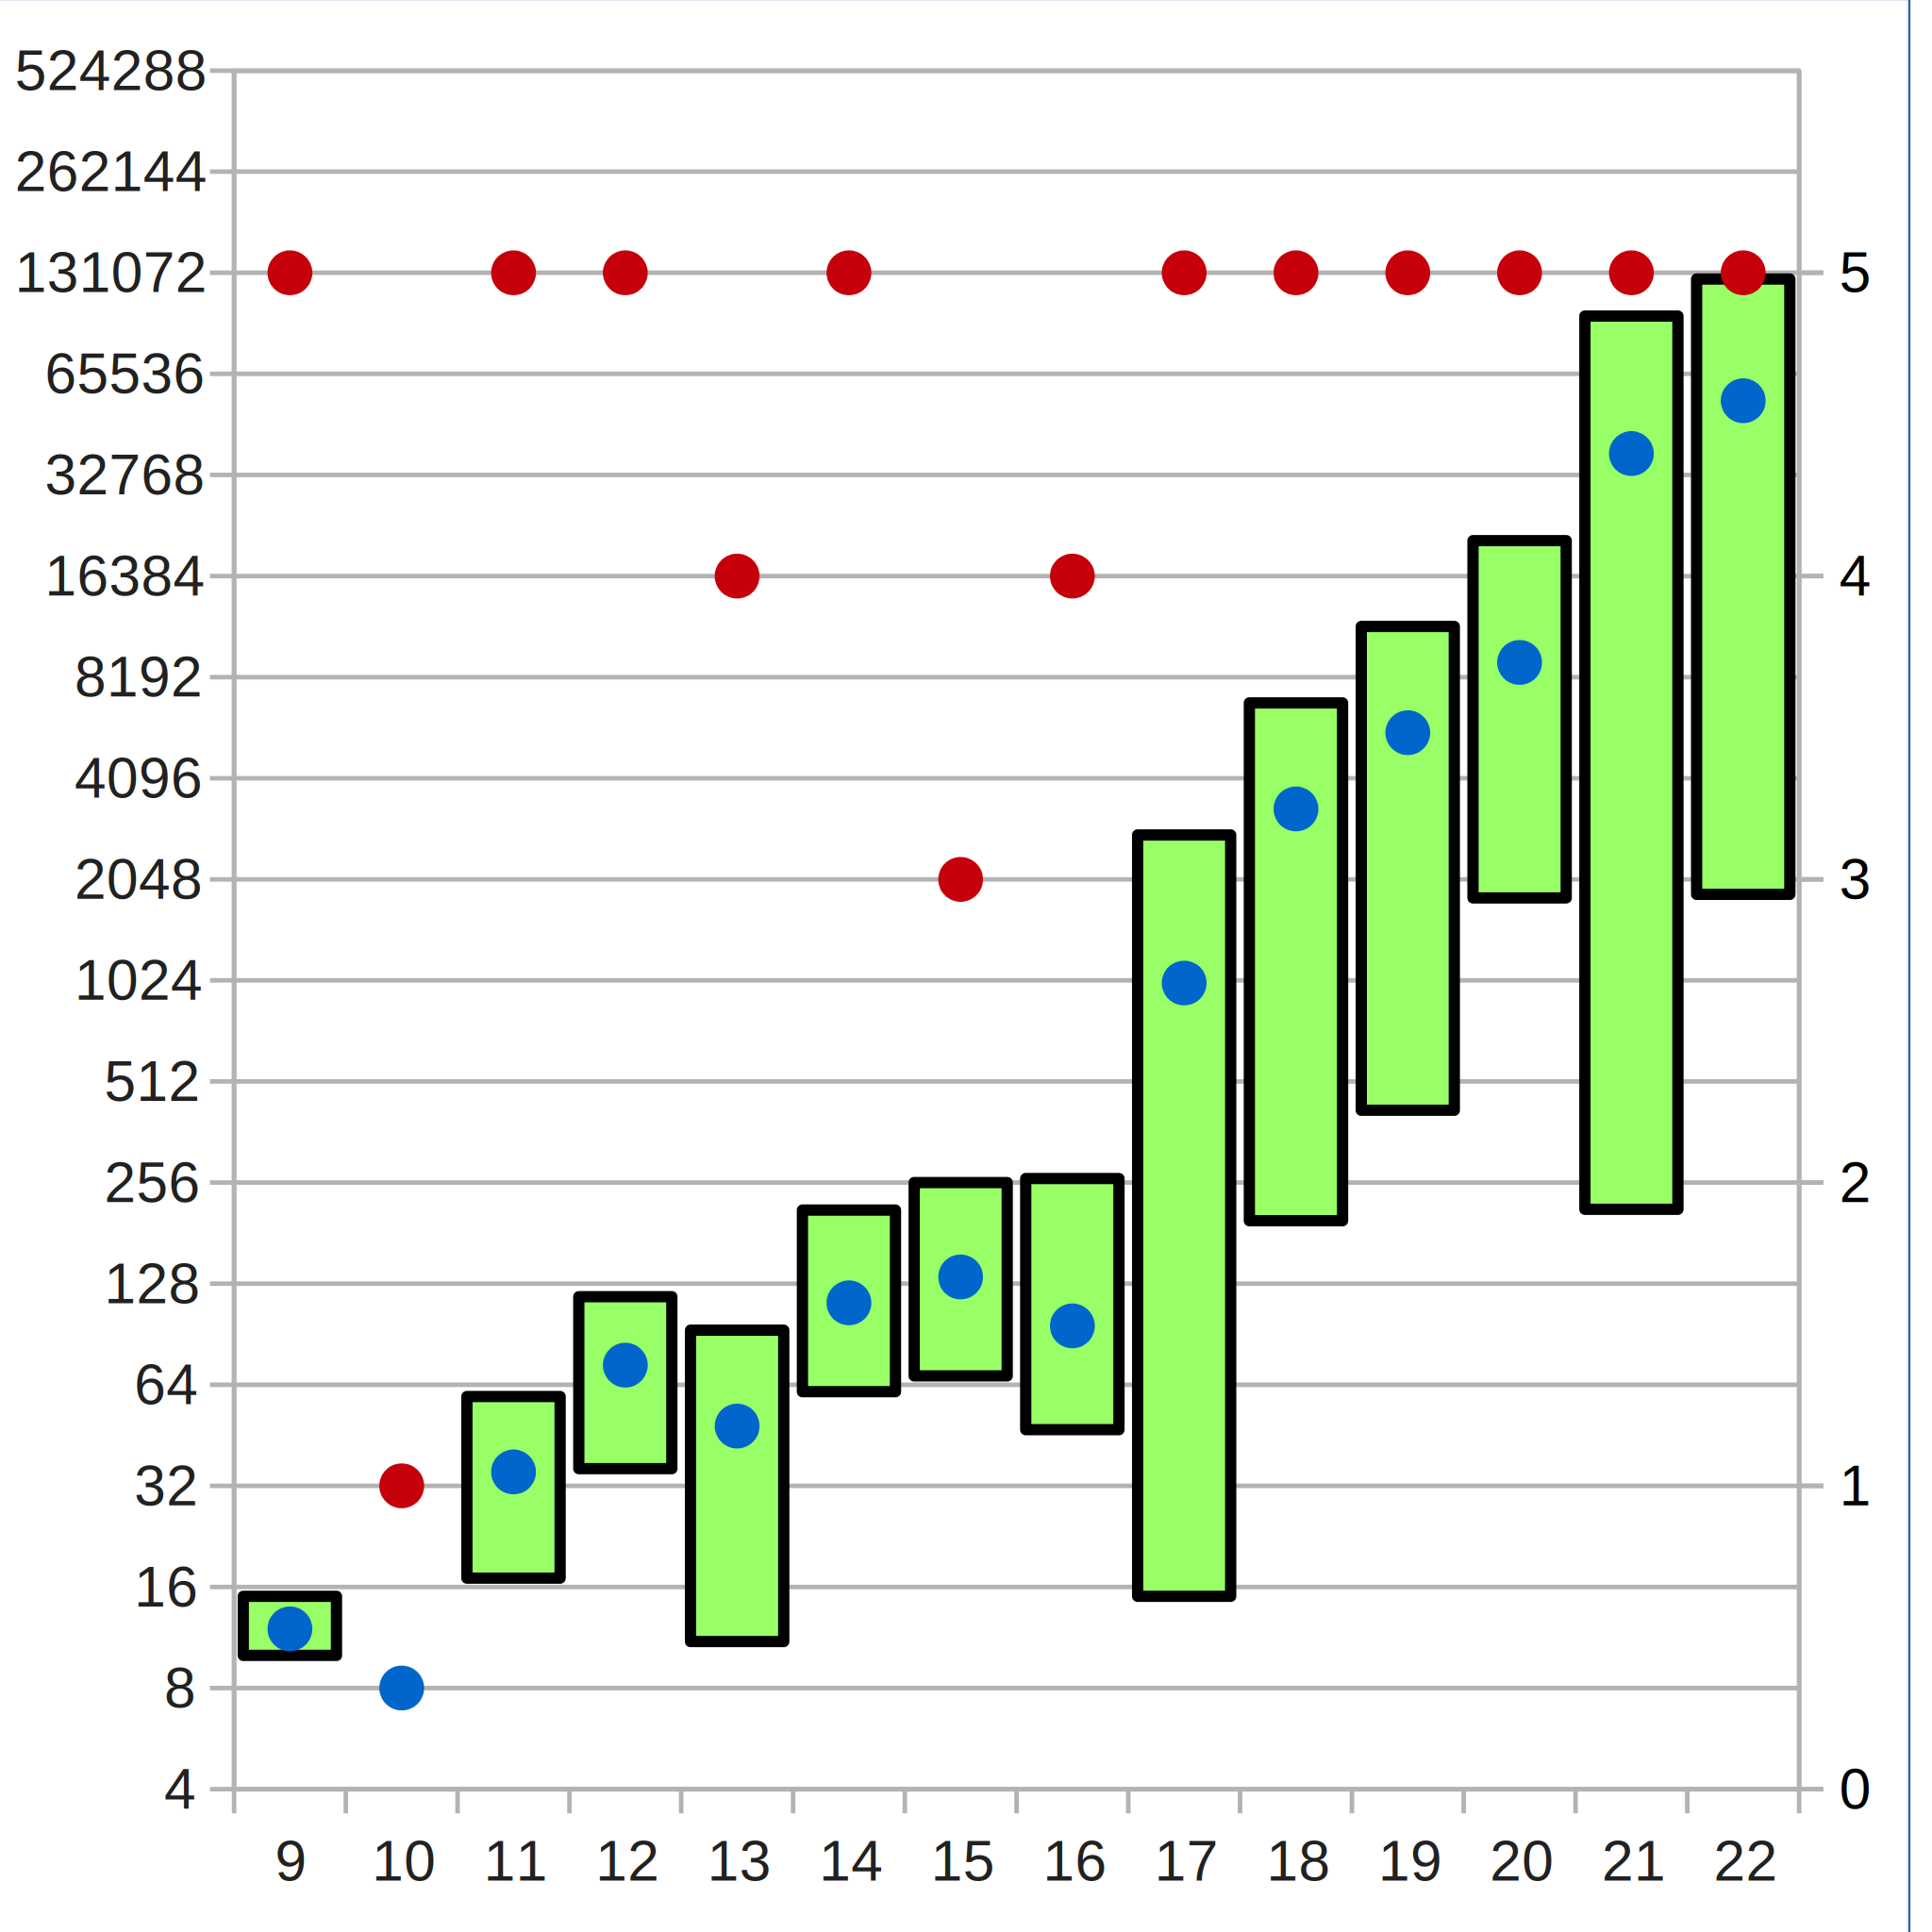
\includegraphics[scale=0.55]{images/data_dist_knf}
  \end{minipage}
  \begin{minipage}[c]{0.09\textwidth}
  ~~
  \end{minipage}
  \begin{minipage}[c]{0.45\textwidth}
  \begin{flushleft}Gesamtdauer mit XOR: 141:34:35\end{flushleft}
  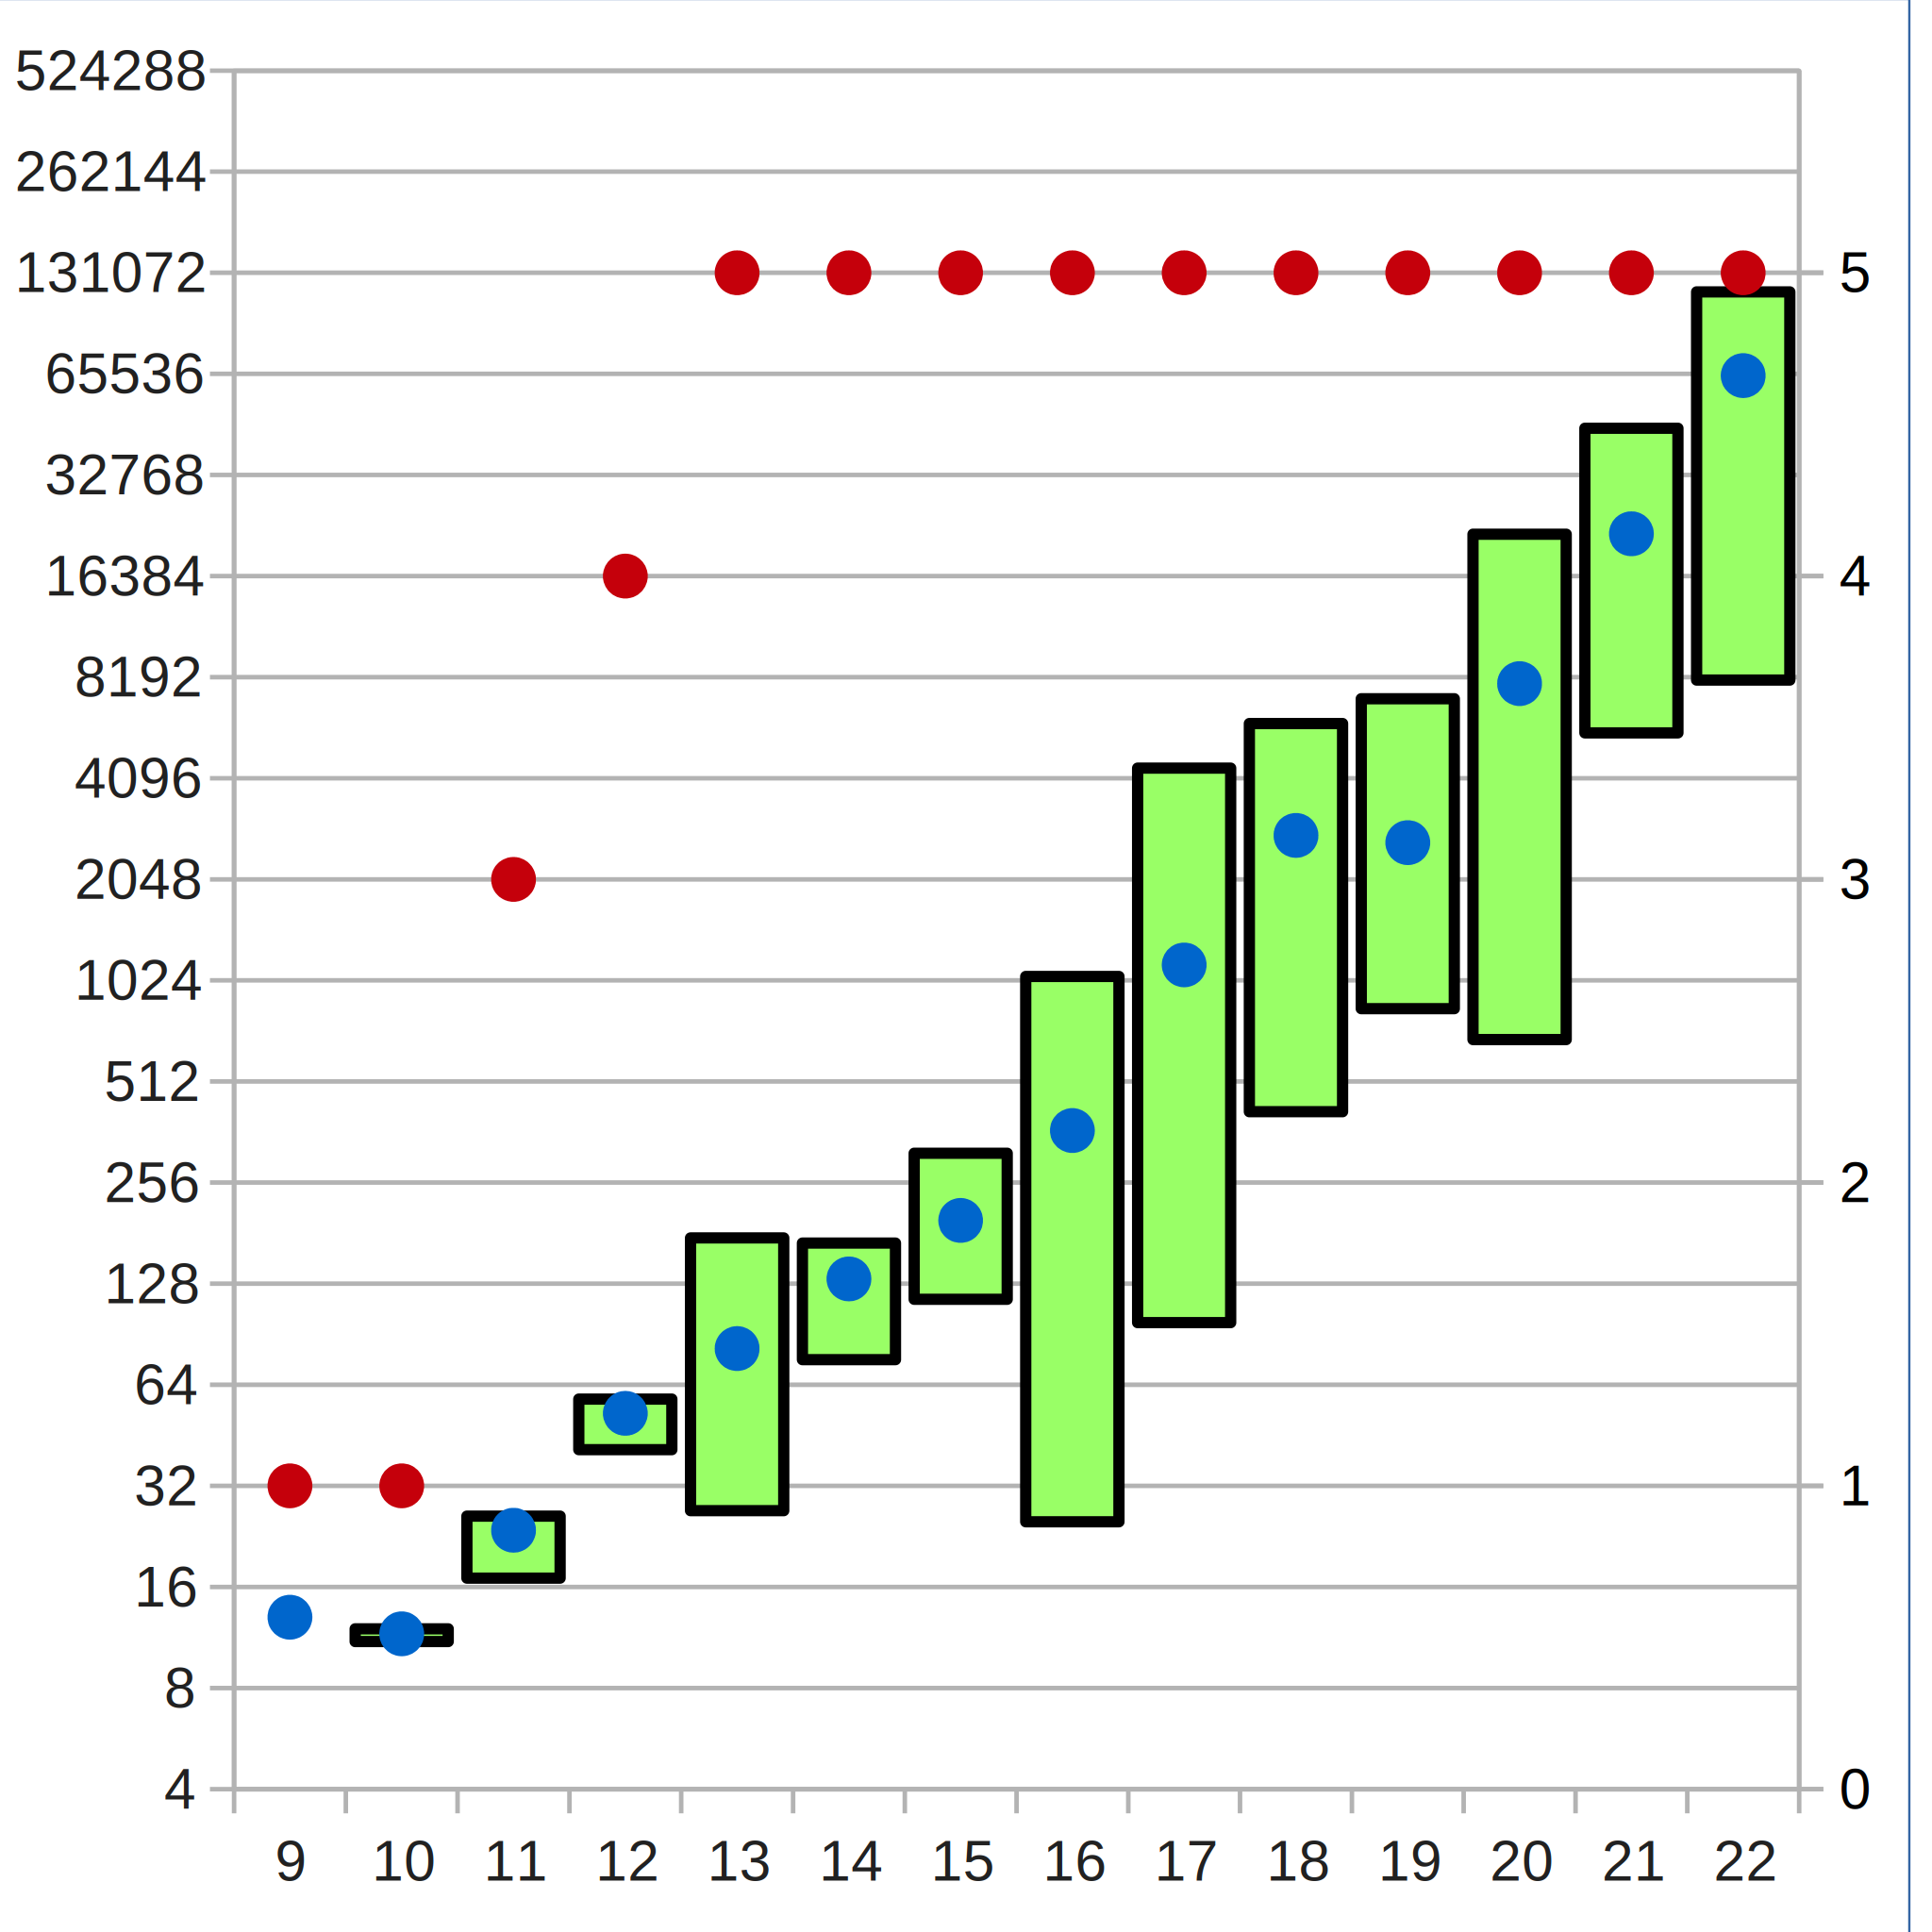
\includegraphics[scale=0.55]{images/data_dist_xor}
  \end{minipage}
  \caption{Ergebnisse mit Distanzklauseln}
  \label{fig:data_dist}
\end{figure}